\chapter{Theoretical Foundations}\label{ch:theoretical-foundations}

This chapter explains the theoretical foundations that are necessary to understand the neural network that was developed in this work.
It first explains how a machine learns from data following with an introduction of a specific neural network architecture, the Transformer.
Finally, a language model based on Transformers is introduced.

% ===============
% LEARNING FROM DATA
% ===============

\section{Learning from Data}

\subsection{Labeled and Unlabeled Data}

When learning from data, it is usually either labeled or unlabeled.
An example of labeled data can be images with a caption, where the image itself is the data and the caption is the label.
For abstractive summarization tasks, data is usually labeled with the source text being the data and the summary of this text being the label.
Unlabeled data can be any data, such as plain images or texts.
Unlike labeled data, the amount of unlabeled data is usually much higher as labeling data is an expensive manual process, while unlabeled data is usually produced as a by-product.
A popular example of unlabeled text data is Wikipedia, which contains over a billion words in English alone \cite{wikipediaStats}. 

%TODO Source?

\subsection{Neural Networks}

\begin{figure}[h]
\centering
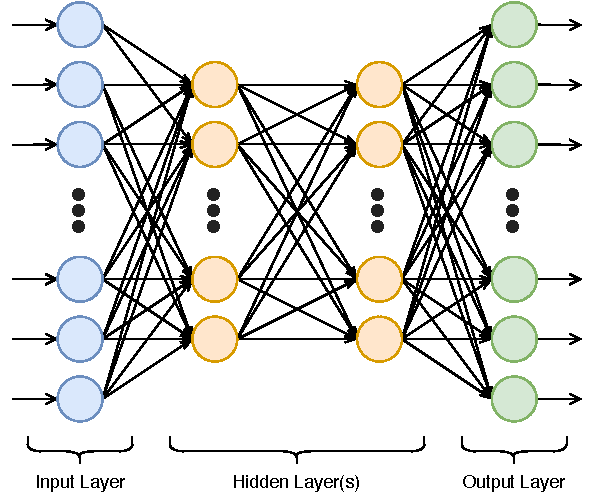
\includegraphics[width=0.45\paperwidth]{figures/neural-network}
\caption{Simple feed-forward neural network with two hidden layers}
\label{fig:neural-network}
\end{figure}

Artificial neural networks are currently a popular and common way to learn from data due to the availability of better hardware and an increasing amount of training data.
A typical neural network consists of neurons that are inspired by real brain neurons and connections between these neurons.
Each neuron can be seen as a function that takes the values of all its predecessor nodes as input and outputs a value that, by itself, is used as the input for its successor nodes.
To compute a node's output, the value $x \in X$ of every predecessor node is multiplied with a weight $w \in W$.
Then, a constant bias, $b$, is added to the sum of these multiplications, and finally an activation function $\Phi$ is applied to this sum as shown in the following equation:
\[
	y = \Phi(\sum_{i=0}^{d}x_iw_i + b)
\]
with $d$ being the number of predecessor nodes and $y$ being the node's output.
For most nodes, the activation function $\Phi$ is usually a nonlinear function that maps its input to values between $-1$ and $1$ or $0$ and $1$.
A popular example of an activation function is sigmoid, which maps negative values to values close to $0$ and positive values to values close to $1$ \cite[p.~4--13]{Aggarwal2018}.

\paragraph{Feed-Forward Networks}

One of the simplest and most common neural network architectures is the feed-forward network.
Such a network consists of multiple layers, where neurons only have predecessors in the previous layer and successors in the next layer.
The first layer with no predecessors is called the input layer as here the actual input for the neural network is used as the node's values.
The last layer with no successors is called the output layer.
The values of the nodes in the output layer are used as the output of the whole network.
Every layer in between these two layers is called a hidden layer.
While the nodes in the hidden layer usually have a nonlinear activation function, nodes in the output layer sometimes have a linear activation function like ReLU if the output is an absolute value. 
Such a network is shown in \cref{fig:neural-network} \cite[p.~17--20]{Aggarwal2018}.

\paragraph{Backpropagation}

When training a network, the goal is to adjust all the weights and biases in a way that the error of the neural network is minimized.
This error is measured with a loss function that computes how different the output of the network for the training data is compared to the desired output (the labels).
Backpropagation is an algorithm that computes how the weights and biases should be adjusted.
The backpropagation algorithm consists of two phases: In the forward phase, a portion (batch) of the training data is fed into the network, and the loss is computed.
In the backward phase, the gradients of the loss function are computed, and then these gradients are used to update the weights of the network.
This processes is repeated multiple times \cite[p.~21--24]{Aggarwal2018}.

% TODO Maybe add an "Overfitting" paragraph

\subsection{Automatic Evaluation}\label{ssec:automatic-evaluation}

Evaluating summaries is essential for multiple reasons (\eg, to monitor progress during training or to compare own results to results from other researchers).
While human evaluation seems like an obvious approach, it is usually not feasible because it is slow and expensive, and results from different people are not always comparable.
Thus, the more common approach is automatic evaluation.
To automatically evaluate summaries, Recall-Oriented Understudy for Gisting Evaluation (ROUGE) \cite{lin-2004-rouge} is widely adapted as it tends to correlate well with human judgments.
In addition, ROUGE supports multiple evaluation metrics.
To report the results achieved in this thesis, the following three metrics are used:
\begin{itemize}
\item \textbf{ROUGE-1}, which calculates the overlap of single words (unigrams) between the candidate summary and the reference summary
\item \textbf{ROUGE-2}, which is similar to ROUGE-1, but instead of using the overlap of single words, it uses word pairs of two (bigrams)
\item \textbf{ROUGE-L}, which uses the longest common subsequence to calculate the score. A subsequence must not be confused with a substring. For the sentences "My favorite name is John Doe" and "My name is Maria Doe," the longest common subsequence would be "My name is Doe," whereas the longest substring would just be "name is."
\end{itemize}

When comparing word overlap, one must differentiate between recall and precision \cite{Ting2010}.
While recall indicates how much information of the reference summary is present in the candidate summary, precision indicates how much of the information in the candidate summary is actually present in the reference summary.
It is common to combine these two measures to a single one, called F1-measure.
It is calculated by the following formula:
\[
	F_1 = 2 \cdot \frac{Recall \cdot Precision}{Recall + Precision}
\]

% ==========
% TRANSFORMER
% ==========

\section{Transformer}\label{sec:transformer}

The Transformer is a neural network architecture for sequence learning that was published in 2017 \cite{1706.03762}.
It achieved new state-of-the-art results for many machine translation tasks while at the same time requiring significantly less training time compared to previous well-performing models.

\subsection{Motivation}\label{ssec:transformer-motivation}

In recent years, recurrent neural networks (RNNs) have been the most common way to solve sequence learning tasks.
However, one of the major downsides of RNNs is their sequential behavior.
To train an RNN, the elements of the input sequence are fed into the neural network one after another.
While the sequence elements are passed through the RNN, a hidden state gets computed at every step, which is part of the input for the next step.
This process is called encoding.
Afterward, the last hidden state of the encoding process is used as an input for the first step of the decoding process.
Because of this, it is not possible to parallelize the training within a training example as the hidden state of the previous step is needed to calculate the output of the current step \cite[p.~2]{1706.03762}.
A simplified RNN for sequence-to-sequence tasks like machine translation is shown in \cref{fig:rnn-visualization}.

\begin{figure}[h]
\centering
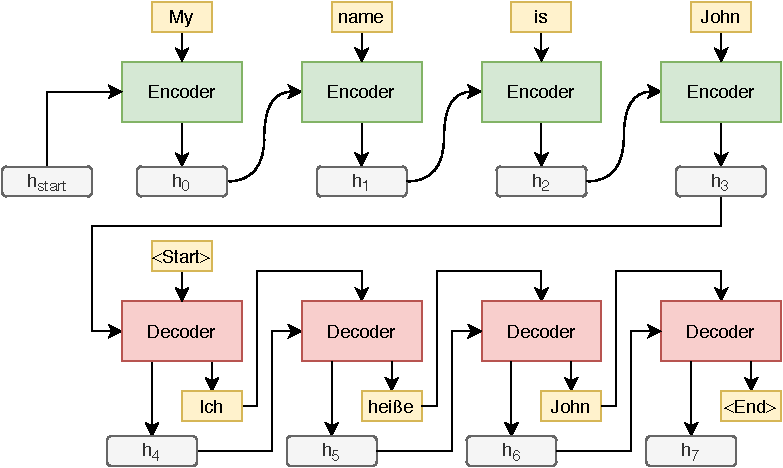
\includegraphics{figures/rnn-visualization}
\caption[Simplified visualization of a sequence-to-sequence RNN network for machine translation]{Simplified visualization of a sequence-to-sequence RNN network for machine translation. The input sequence is fed into the encoder with one word for each step. The final hidden state, which is computed in the last encoding step, is used as input for the first decoding step. The initial hidden state, $h_{start}$, can be initialized as a vector of zeros or learned during training.}
\label{fig:rnn-visualization}
\end{figure}

Another problem with RNNs is the long distance, that information must "travel" before it is used. % TODO Illustrate this long "travel" distance
Information that was encoded into the hidden state must pass through multiple encoding and decoding steps, before it is finally used in one of the decoding steps.
Besides having the hidden state as an information bottleneck, this also makes it very hard for the network to learn long range dependencies because of the problem of vanishing or exploding gradients \cite{Hochreiter01gradientflow}. % TODO Maybe briefly explain the problem
Modern variants of RNNs, like the long short-term memory (LSTM) architecture \cite{Hochreiter1997}, try to mitigate these effects but are not able to fully eliminate them.
A fairly recent solution to this problem is the attention mechanism that was first proposed in 2014 \cite{1409.0473}.
It allows the network in the decoding stage to retrieve information from any hidden state that was computed during the encoding stage.
This eliminates the issue of learning long range dependencies.

The Transformer network takes advantage of the attention mechanism while avoiding the recurrence of RNNs to achieve faster training and allow for more parallelization.

\subsection{Model Architecture}\label{ssec:transformer-model-architecture}

Just like sequence-to-sequence RNNs, the Transformer consists of an encoder and a decoder that both have multiple stacks of layers.

\begin{figure}[h]
\centering
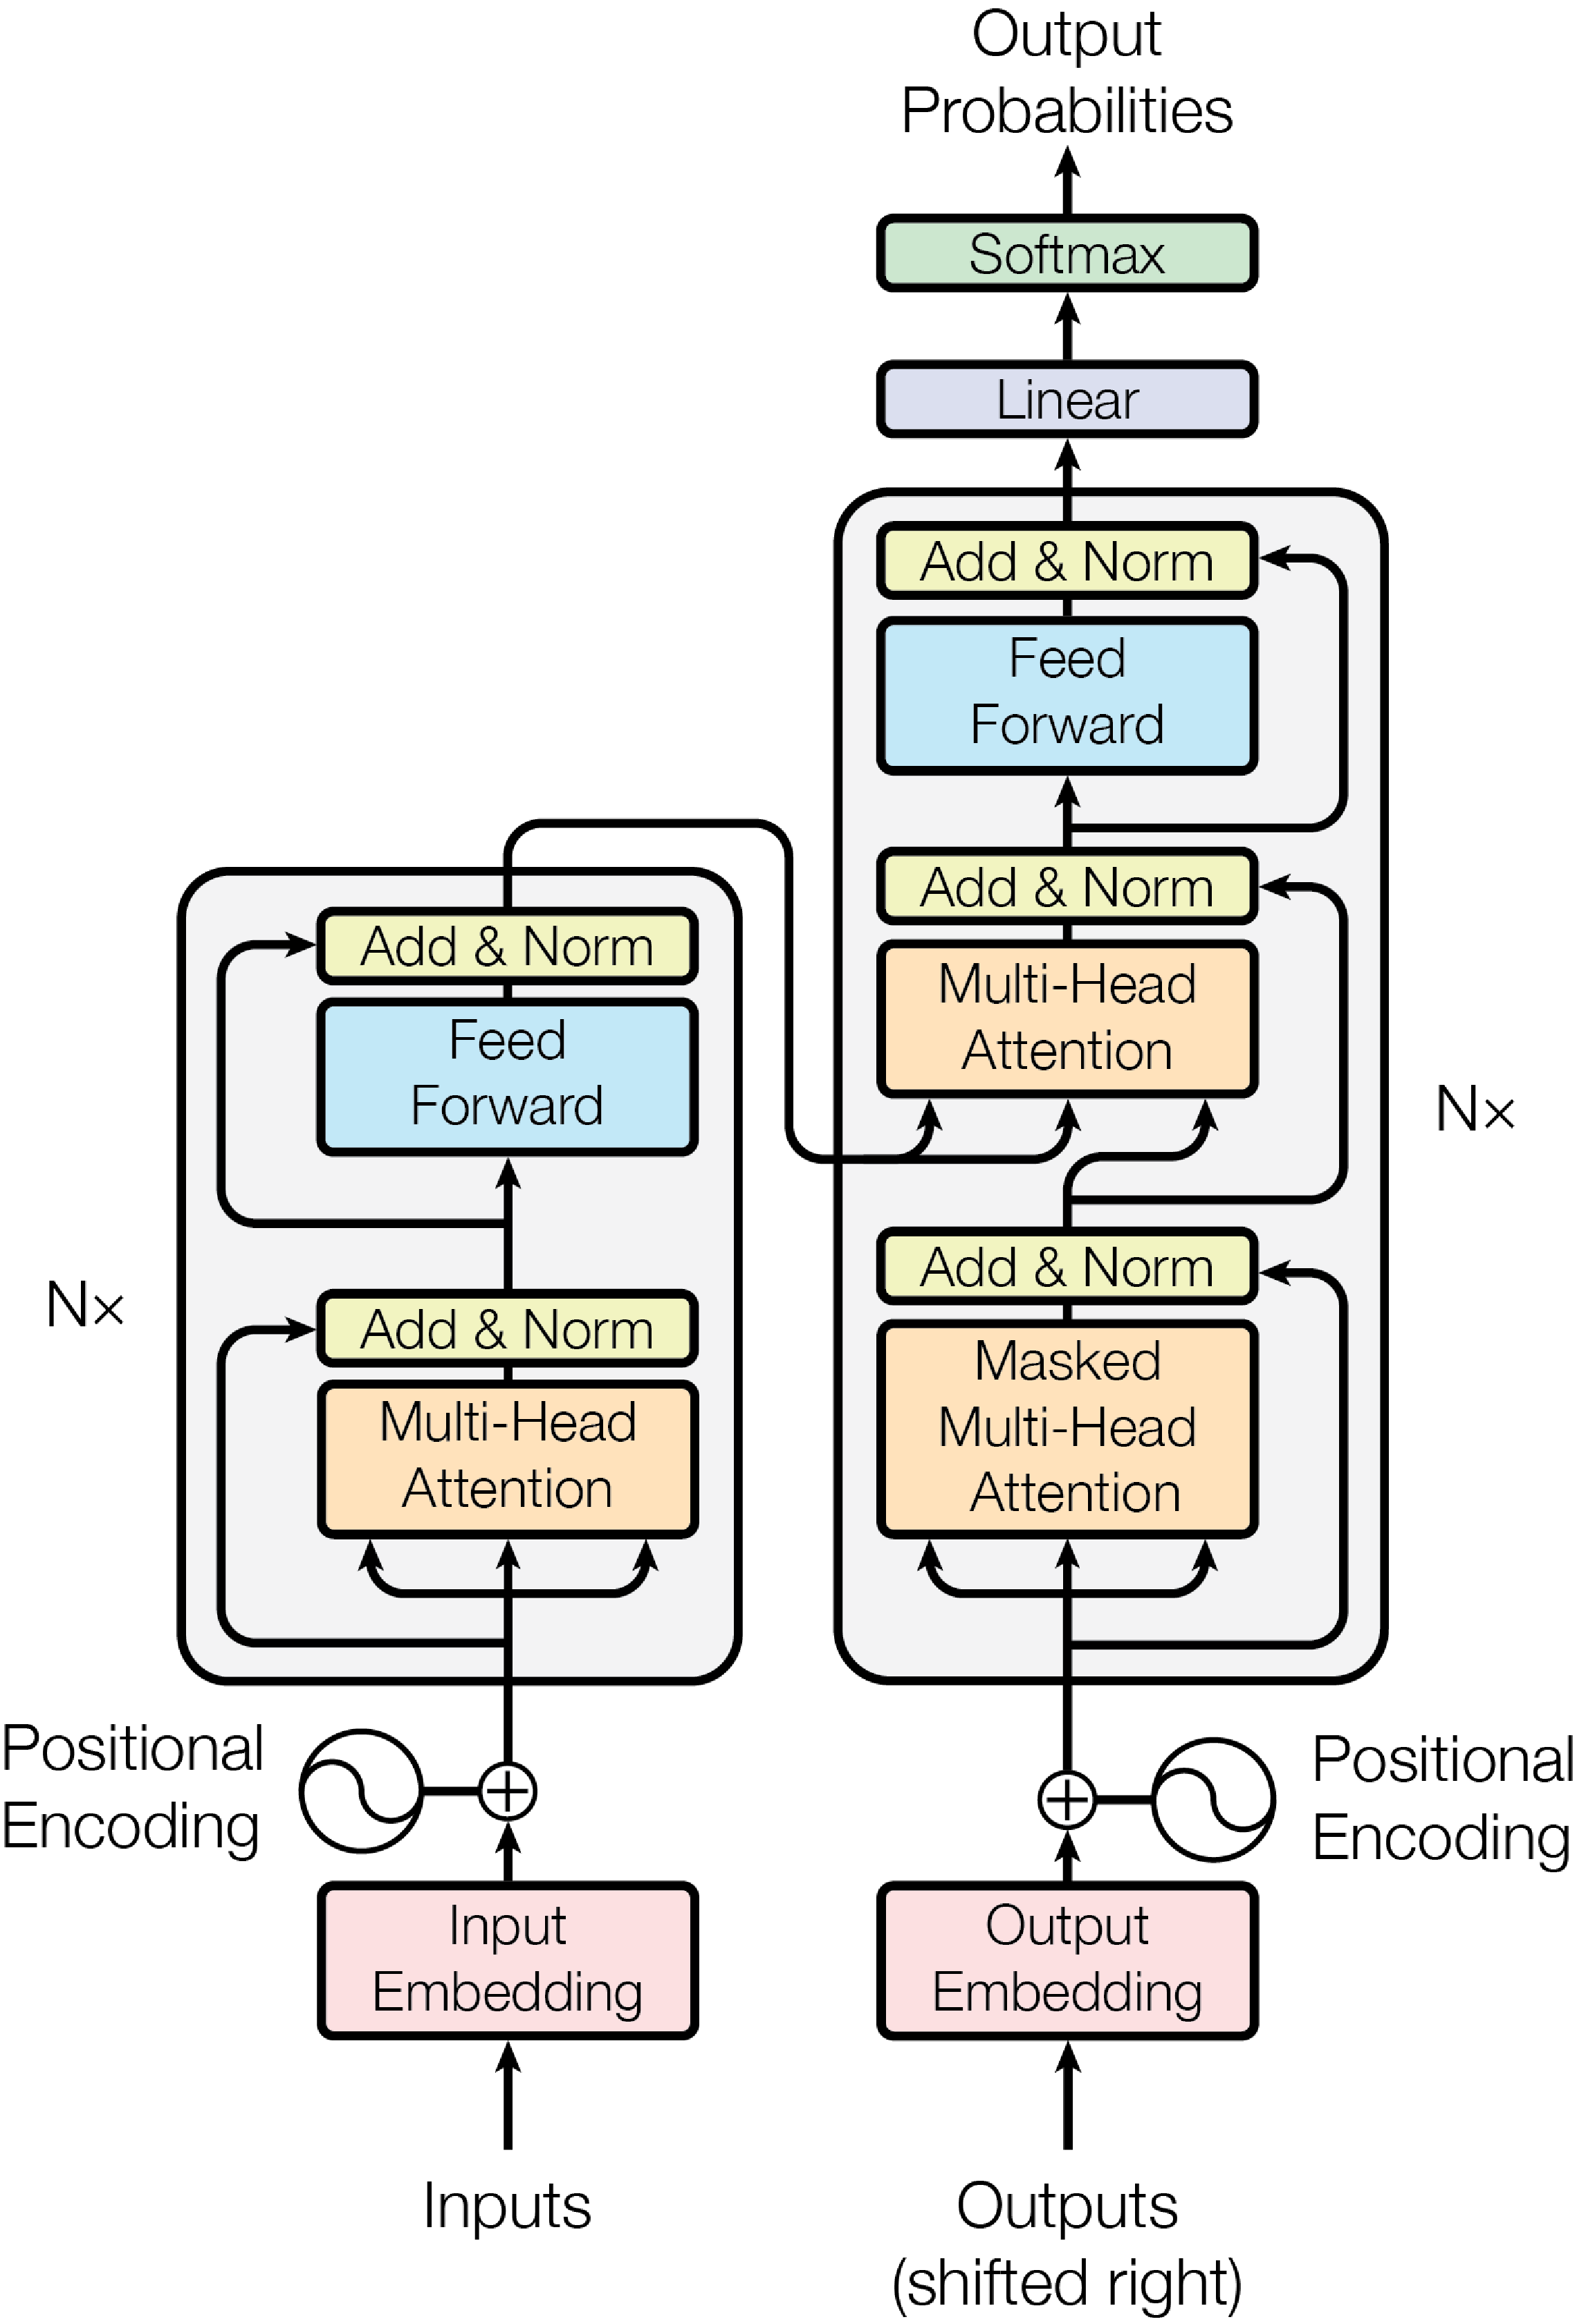
\includegraphics{figures/transformer-model}
\caption[Model architecture of a Transformer]{Model architecture of a Transformer \cite[p.~3]{1706.03762}}
\label{fig:transformer-model}
\end{figure}

An encoder layer consists of two sublayers.
The first sublayer is a multi-head self-attention mechanism, which is described later in this section.
The second sublayer is a position-wise\footnote{The identical network is applied to each position separately \cite[p.~5]{1706.03762}.} fully connected feed-forward network.
Both sublayers have residual connections \cite{1512.03385} around them that are followed by layer normalization \cite{1607.06450}.
The outputs of the layers of the Transformer base model have $d_{model}=512$ dimensions and $d_{model}=1024$ for the big model \cite[p.~9]{1706.03762}.

An encoder layer has a similar structure but with one additional sublayer and a slight modification of the multi-head self-attention sublayer.
The new sublayer attends to the output of the encoder.
The multi-head self-attention sublayer is masked to prevent it from attending to future words \cite[p.~3]{1706.03762}.

In the original Transformer, $N = 6$ stacked encoder and decoder layers are used for both the base and the big model.
The complete architecture of the Transformer is visualized in \cref{fig:transformer-model}.

The inputs are simple learned embedding vectors of dimension $d_{model}$ that are concatenated with a fixed positional embedding \cite[p.~5--6]{1706.03762}.
These fixed input embeddings encode the position of the sequence elements as this information is otherwise no longer accessible to the network because of the missing recurrence.
The positional encoding is calculated with sine and cosine functions of different frequencies:
\begin{align*} 
	PE_{(pos,2i)} & = sin(pos/10000^{2i/d_{model}}) \\
	PE_{(pos,2i+1)} & = cos(pos/10000^{2i/d_{model}})
\end{align*}

This encoding allows the network to obtain information about the absolute and relative position of each element.
\Cref{fig:positional-encoding-sine-cosine} illustrates the embedding for some dimensions.
It is clearly visible how each position has a different positional embedding.

For the outputs, a learned linear transformation and a softmax function are used to compute next-token probabilities \cite[p.~5]{1706.03762}.

\begin{figure}[h]
\centering
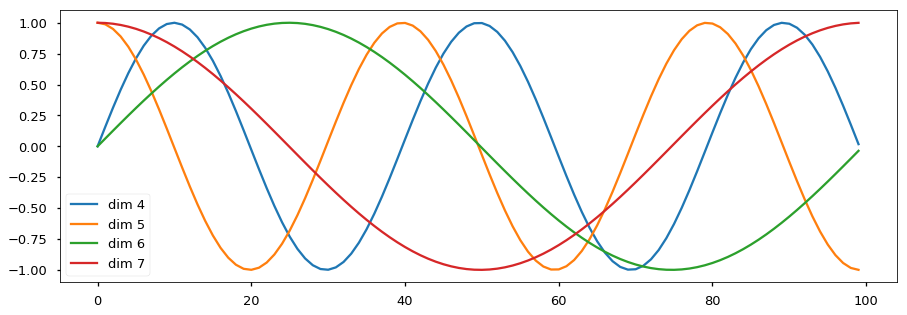
\includegraphics[width=0.7\paperwidth]{figures/positional-encoding-sine-cosine}
\caption[Visualization of positional encoding with sine and cosine]{Visualization of positional encoding with sine and cosine \cite{annotated.transformer}}
\label{fig:positional-encoding-sine-cosine}
\end{figure}

\paragraph{Attention}

\begin{figure}[h]
\centering
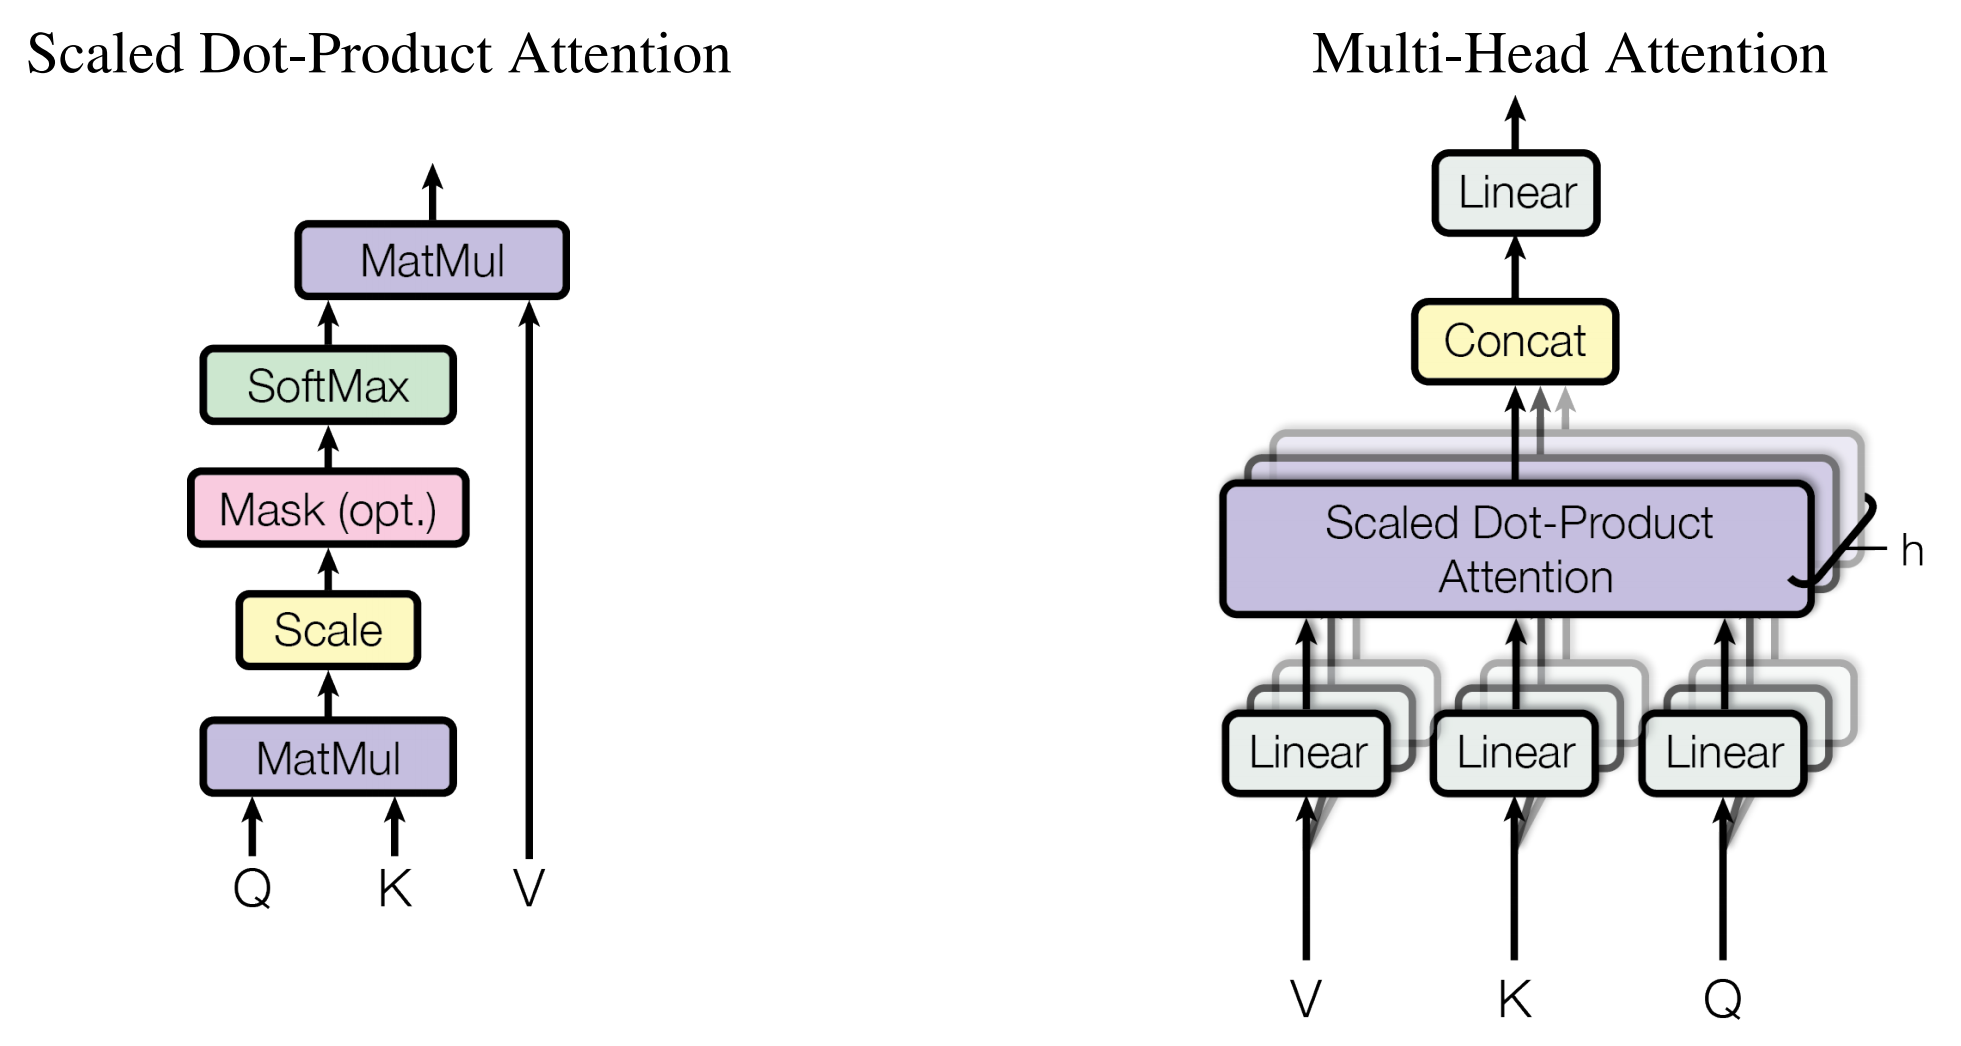
\includegraphics[width=0.7\paperwidth]{figures/scaled-dot-product-multihead-attention}
\caption[Visualization of scaled dot-product attention and multi-mead attention]{Visualization of scaled dot-product attention and multi-head attention \cite[p.~4]{1706.03762}}
\label{fig:scaled-dot-product-multihead-attention}
\end{figure}

The Transformer attention consists of query, key, and value vectors.
The query vectors are used to select values by their corresponding keys.
The Transformer implements this as a scaled dot-product attention, wherein queries and keys have the dimension $d_k$ and the values the dimension $d_v$.
To calculate the attention, the following formula is used:
\[
	\textrm{Attention}(Q,K,V) = \textrm{softmax}(\dfrac{QK^T}{\sqrt{d_k}})V
\]
where $Q$, $K$, and $V$ are matrices that contain multiple sets of queries, keys, and values \cite[p.~3--4]{1706.03762}.
Masking for the decoder layer is easily performed by setting the input values of the softmax function to $-\infty$ if they are not allowed.

Unlike normal attention, the Transformer uses multi-head attention.
This means that instead of having a single attention function, the queries, keys, and values are linearly projected with learned linear projections \cite[p.~4--5]{1706.03762}.
After performing the attention function on the projected matrices, they are concatenated and projected again.
The dimension of each learned linear projection is the model's dimension $d_{model}$ divided by the number of attention layers $h$.
\Cref{fig:scaled-dot-product-multihead-attention} shows both the scaled dot-product attention (left) and the multi-head attention (right).

\subsection{Advantages}

As described in \cref{ssec:transformer-motivation}, the Transformer allows for significantly more parallelization than RNNs because of the absence of sequential behavior within one training example.
This yields much faster and less expensive training compared to previous state-of-the-art models for machine translation.
The big Transformer model is trained for 3.5 days on 8 P100 GPUs and the base Transformer model for just 12 hours \cite[p.~7]{1706.03762}. 
In comparison, the first RNN network to utilize attention took between 109 and 252 hours for training \cite[p.~14]{1409.0473}.

\subsection{Disadvantages}

Transformer networks tend to get very large and require a large amount of memory, especially for longer sequence lengths as the self-attention connects every position with every other position in the sequence.
This results in quadratic complexity for the sequence length.
As a solution, the authors of the Transformer suggest limiting the self-attention to the neighbors of each position \cite[p.~6--7]{1706.03762}.  
The more recent Reformer \cite{kitaev2020reformer} solves this issue by using locality-sensitive hashing to reduce the complexity from $O(L^2)$ to $O(L)$.

% ====
% BERT
% ====

\section{BERT}\label{sec:bert}

Bidirectional Encoder Representations from Transformers (BERT) is a general-purpose language model that was released by Google AI researchers in mid-2018.
It broke several records for natural language processing benchmarks \cite[p.~5--7]{devlin2018bert}, such as  SQuAD v1.1 \cite{rajpurkar-etal-2016-squad} and GLUE \cite{1804.07461}.

\subsection{Motivation}

It has been shown that results for many natural language processing tasks can be improved with the help of language models.
The most famous among them are OpenAI's GPT-2 \cite{radford2019language} and ELMo \cite{1802.05365}.
The benefit of language models is that most of them can be trained on unlabeled data like Wikipedia articles or large book corpora.
This allows them to learn from a huge amount of data as there is no need for time-consuming labeling of the training data and any texts can be used.
By pretraining them on normal texts, the networks can get a general sense of natural language, which can then be used for more specific tasks.

% TODO Not sure if I keep using this or create an own one / just remove it
\begin{figure}[h]
\centering
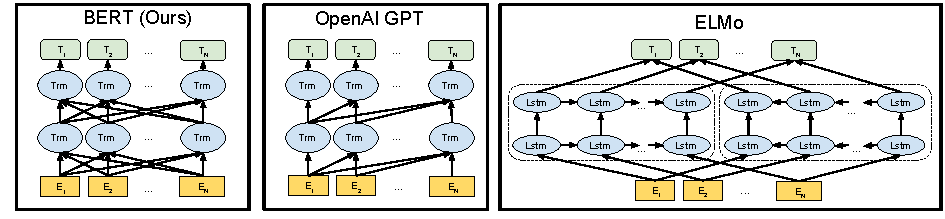
\includegraphics[width=0.7\paperwidth]{figures/bert-gpt2-elmo-model-comparison}
\caption[Visualization of the different model architectures]{Visualization of the different model architectures \cite[p.~13]{devlin2018bert}}
\label{fig:bert-gpt2-elmo-model-comparison}
\end{figure}

What is new about BERT compared to other models like GPT-2 is that it is the first deeply bidirectional language model that takes advantage of the whole context around a word.
OpenAI's GPT-2 uses a left-to-right Transformer decoder \cite[p.~4]{radford2019language}, which only allows it to "look" at the words to the left when generating a representation for an input token.
For example, with a sentence that starts with "The lighter," the network can only look at these two words to generate a representation for the word "lighter."
However, the word can have completely different meanings depending on the whole sentence (\eg, "The lighter is an easy tool for making fire" compared to "The lighter shade of red looks better than the darker one"). 
ELMo compensates for this issue by training two LSTMs, one being a normal forward LSTM (left-to-right) and the other one being a backward LSTM (right-to-left), which is given the input sequence in reverse \cite[p.~2--3]{1802.05365}.
Afterward, it concatenates the representations of these two LSTMs to get a semi-bidirectional representation.
\Cref{fig:bert-gpt2-elmo-model-comparison} presents the different architectures.

\subsection{Model Architecture}

At its core, BERT is just a Transformer encoder, as described in \cref{ssec:transformer-model-architecture}.
What is innovative about BERT's architecture is mainly how it is trained and how the inputs and outputs are represented.

\paragraph{Input and Output Representations}

BERT's input is applicable to many different natural language processing tasks.
It allows the inputs of either one sentence or a pair of two sentences.\footnote{In the context of BERT, a sentence does not refer to an actual linguistic sentence, but an arbitrary span of contiguous text \cite[p.~4]{devlin2018bert}.}
Texts are tokenized by using WordPiece embeddings with a vocabulary of 30,000 tokens. 
WordPiece embeddings have the advantage of not needing out-of-vocabulary tokens like the more traditional word embeddings.
Every input sequence starts with a special \texttt{[CLS]} token, and every sentence ends with a special \texttt{[SEP]} token.
In addition to the token embeddings, the input consists of two more types of embeddings.
The first ones are learned segment embeddings that indicate if a token belongs to the first or the second token.
The second ones are position embeddings that help the network to understand the positions of each token in the sequence.
Unlike the original Transformer, BERT does not use fixed positional embeddings but learned ones.
Finally, these three embeddings are concatenated to form the actual input for the network as shown in \cref{fig:bert-input-representation}.

\begin{figure}[h]
\centering
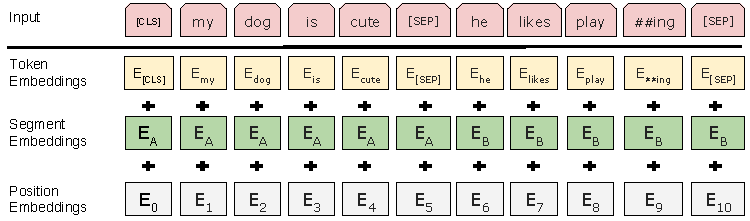
\includegraphics{figures/bert-input-representation}
\caption[BERT input representation]{BERT input representation \cite[p.~5]{devlin2018bert}}
\label{fig:bert-input-representation}
\end{figure}

Depending on the task to perform, there are different ways to use the final hidden states of the BERT Transformer network.
For sentence classification tasks, the \texttt{[CLS]} token representation can be used.
This work uses the final hidden states for every single input token, as the decoder should have access to the presentation of every input token.
For the simpler extractive summarization task, which is basically a kind of sentence classification in which each sentence is either classified as \texttt{"include in summary"} or \texttt{"do not include in summary,"} it is sufficient to only use the final hidden state of the \texttt{[CLS]} token. 
\cite{1903.10318} proposes a small input variation for BERT that inserts multiple \texttt{[CLS]} tokens into the input sequence to later use them for extractive summarization.

\paragraph{Pretraining Objectives}

BERT is pretrained with two different tasks \cite[p.~4--5]{devlin2018bert}.
For the first task, the network is given a sentence with 15\% of its WordPiece tokens randomly masked.
An example of masking is shown in \cref{fig:bert_masking_example}.

\begin{figure}[h]
\begin{lstlisting}[numbers=none]
Input: the man went to the [MASK1] . he bought a [MASK2] of milk.
Labels: [MASK1] = store; [MASK2] = gallon
\end{lstlisting}
\caption[Masked input example]{Masked input example \cite{bertGithub}}
\label{fig:bert_masking_example}
\end{figure}

The task of the network is to predict the masked tokens.
This task requires the network to learn to take the context of a word into consideration.

For the second task, the network is given two sentences.
The network must then predict if the second of these two sentences comes after the first one in the original text or if it is just a randomly selected sentence from any other text.
An example of next-sentence prediction is shown in \cref{fig:bert_next_sentence_example}.

\begin{figure}[h]
\begin{lstlisting}[numbers=none]
Sentence A: the man went to the store .
Sentence B: he bought a gallon of milk .
Label: IsNextSentence

Sentence A: the man went to the store .
Sentence B: penguins are flightless .
Label: NotNextSentence
\end{lstlisting}
\caption[Next-sentence prediction example]{Next-sentence prediction example \cite{bertGithub}}
\label{fig:bert_next_sentence_example}
\end{figure}

Ideally, this helps the network to understand the relationship between two sentences.
However, this task has been shown to be too simple for the network as it is easier for it to just learn if the topics of two sentences match instead of understanding the real relationship of the sentences.
To make the task harder, newer successors of BERT such as ALBERT use slightly changed training objectives, like sentence-order prediction \cite[p.~3]{1909.11942}, in which the goal is to predict which of two given sentences comes first.
This allows the network to better learn the relationship between sentences instead of just detecting matching topics.

Pretraining is usually expensive.
The training of the pretrained BERT models was performed for four days on four Cloud TPUs for BERT\textsubscript{BASE} and 16 Cloud TPUs for the larger model, BERT\textsubscript{LARGE}, with each Cloud TPU having four TPU chips \cite[p.~13]{devlin2018bert}.
However, it is only necessary to do pretraining once.

\paragraph{Fine-Tuning}

After the unsupervised pretraining, the network can be fine-tuned for a specific task.
This is done by just training a full network on the desired task for a short time.
Fine-tuning is far less expensive than pretraining and can usually be done in less than one hour on a single Cloud TPU or a few hours on a normal GPU \cite[p.~5]{devlin2018bert}.

% TODO Either summarize this chapter or lead to the next chapter
